\documentclass[main.tex]{subfiles}
\begin{document}
To begin with, we performed the ethnography study on why would a driver  need to use the SEDA. Since the SEDA aimed for a car driver, we observed about what available at in-car intelligent systems. Nowadays, cars in their top of the range models were equipped with relatively good driving assist technology such as Blind Sport Checking, Lane Departure Warning, Forward Collision Warning, Autonomous Cruise Control or Adaptive Cruise Control, Hand-free phone and voice command ability, Heads-up Display (HUD) or Active Display and so on. In our study, we managed to go through detail feature comparison on 2014 Mazada3 Astina model and 2015 Jeep Cherokee Trailhawk model. We performed the actual test driving on these cars models, comparison of manufacturer printed catalog and observing various user reviews available through Internet. The outcome of this observation survey concluded that most of the intelligent features were available only at the top of the range model in most car brands. However, we also conducted empirical survey  on potential car buyers and found that most people chose to buy lower range models. This key reason was to trade off with top of the range cars lose the most value \cite{carbuy1, carbuy2}. It was unfortunate that those advanced in-car intelligence feature only available in such top range models. Intuitively, this gave us a hunch on how the SEDA might fill in the gap.
\\

\begin{figure}
\caption{SEDA Brainstorm 1}
\centering
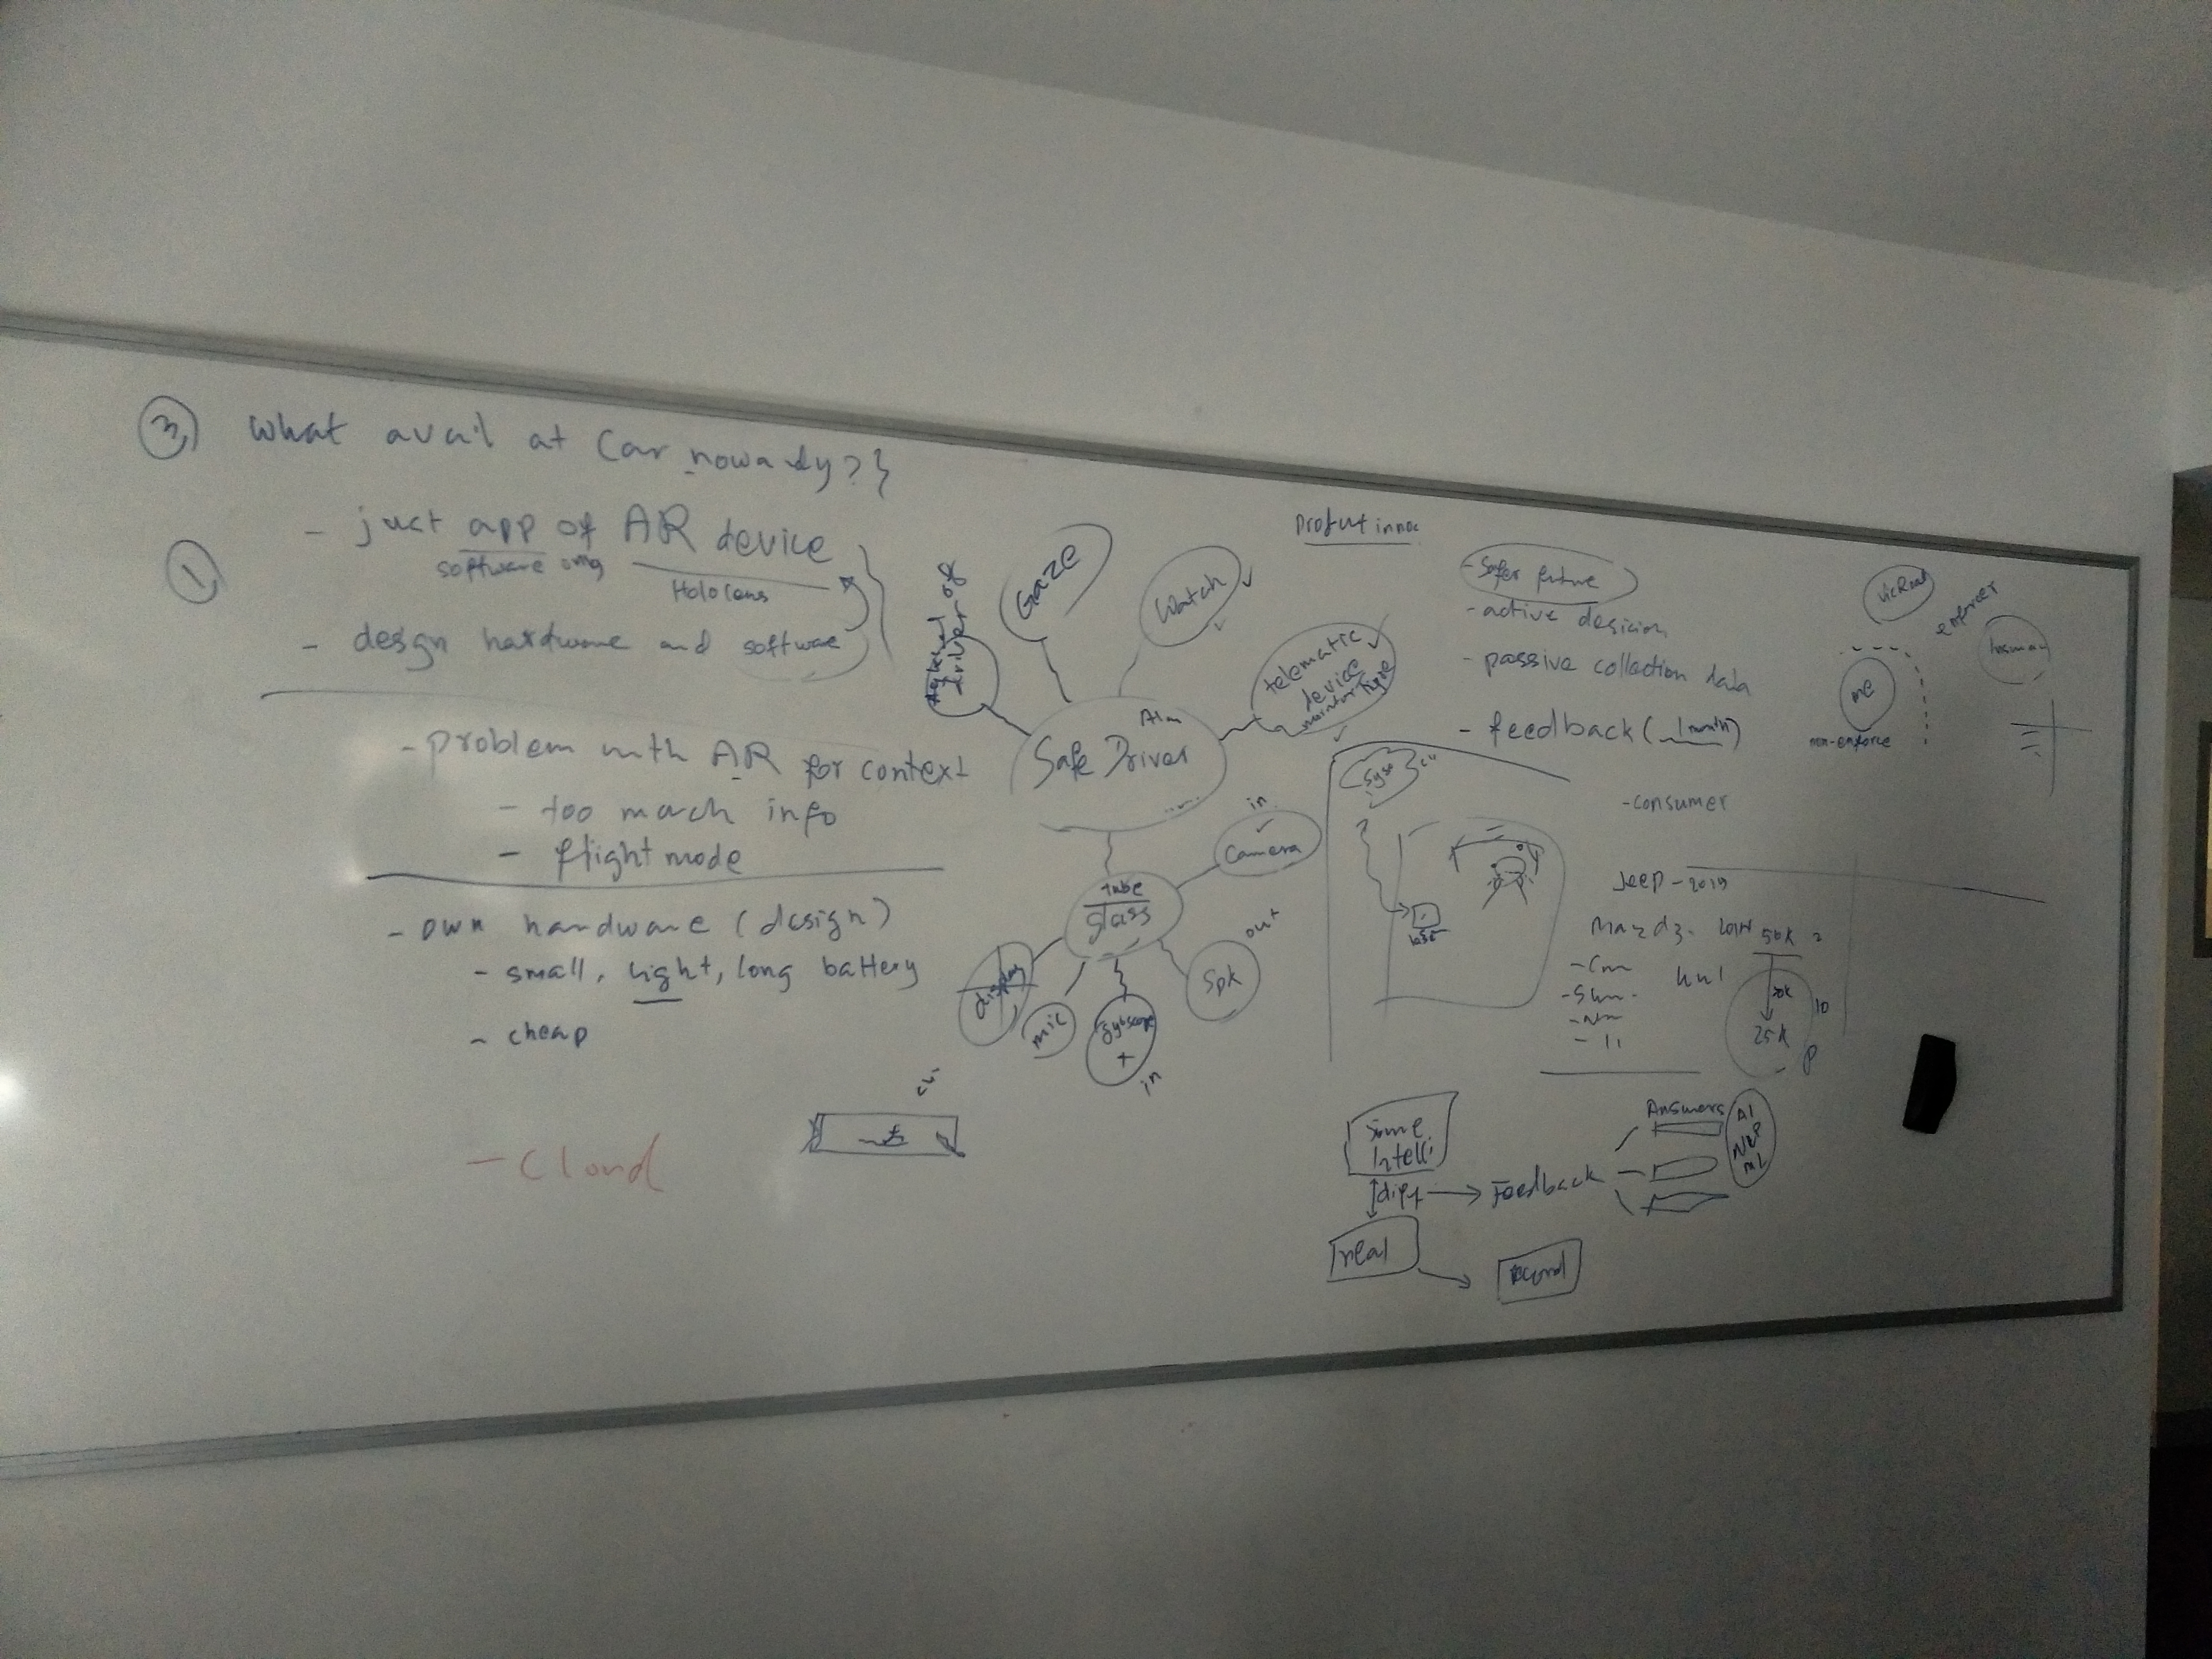
\includegraphics[width=\columnwidth]{brainstorm1}
\end{figure}

Our next research went onto the trend with Augmented Reality (AR) technology and the AR gadgets available in market. One of our initial hypothesis was that the SEDA could be just an app\footnote{eye-wear mobile application} for Microsoft Hololens or Google Glass, for example. In fact, we also thought of SEDA as a pure software system only that could integrate into the existing car system as a smart feature and/or we made an assumption such that a driver might be as well a user of AR eye-wear gadgets or smart glasses. However, this could lead us into tight coupling with a specific car brand and AR gadget where we might only have little of control over. Furthermore, when we observed the available AR gadgets, most of them were in a form of eye-wear product and composed of \textbf{visual} augmented reality. In contrast, we thought of the SEDA as an \textbf{audio} augmented reality, i.e. thought of it as Apple Siri or Google Home technology. Empirically, the audio only augmented reality was preferable for any driving situation where a driver eye had to fix on the road.
\\

\begin{figure}
\caption{SEDA Brainstorm 2}
\centering
\includegraphics[width=\columnwidth, height=10cm]{brainstorm2}
%\includegraphics[scale=0.5]{brainstorm2}
\end{figure}

\end{document}